\section{System models}
\subsection{Dataflow Graph (DFG)}
\begin{figure}[h]
	\begin{center}
		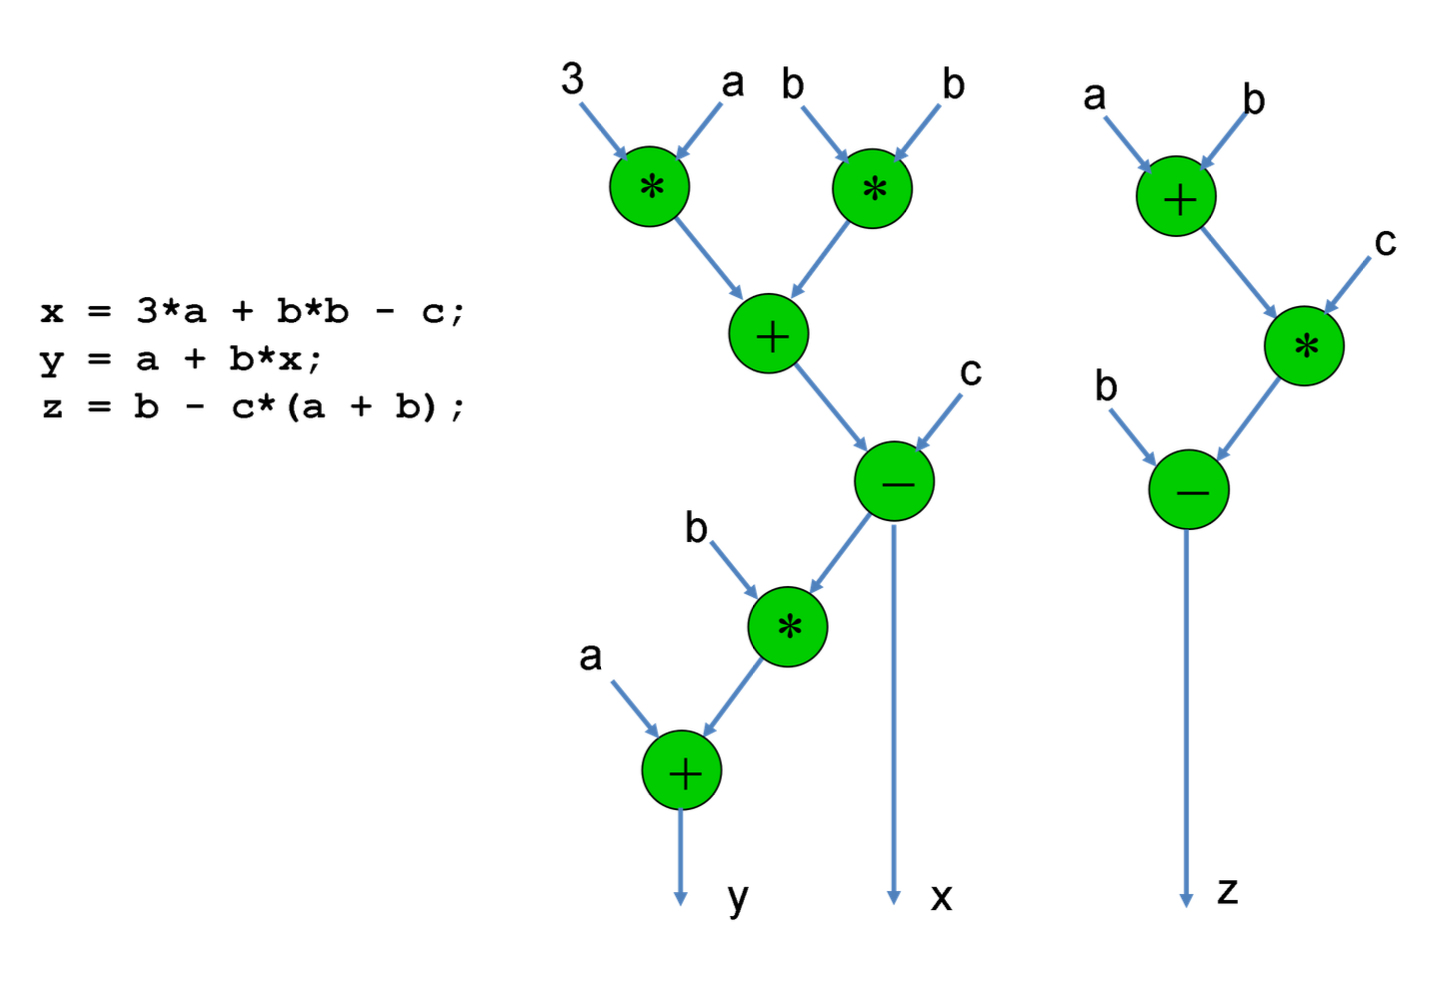
\includegraphics[width=0.5\textwidth]{images/DFG.png}
		\caption{Data Flow Graph}
		\label{fig:DFG}
	\end{center}
\end{figure}

\subsection{Control flow graph (CFG)}
\begin{figure}[h]
	\begin{center}
		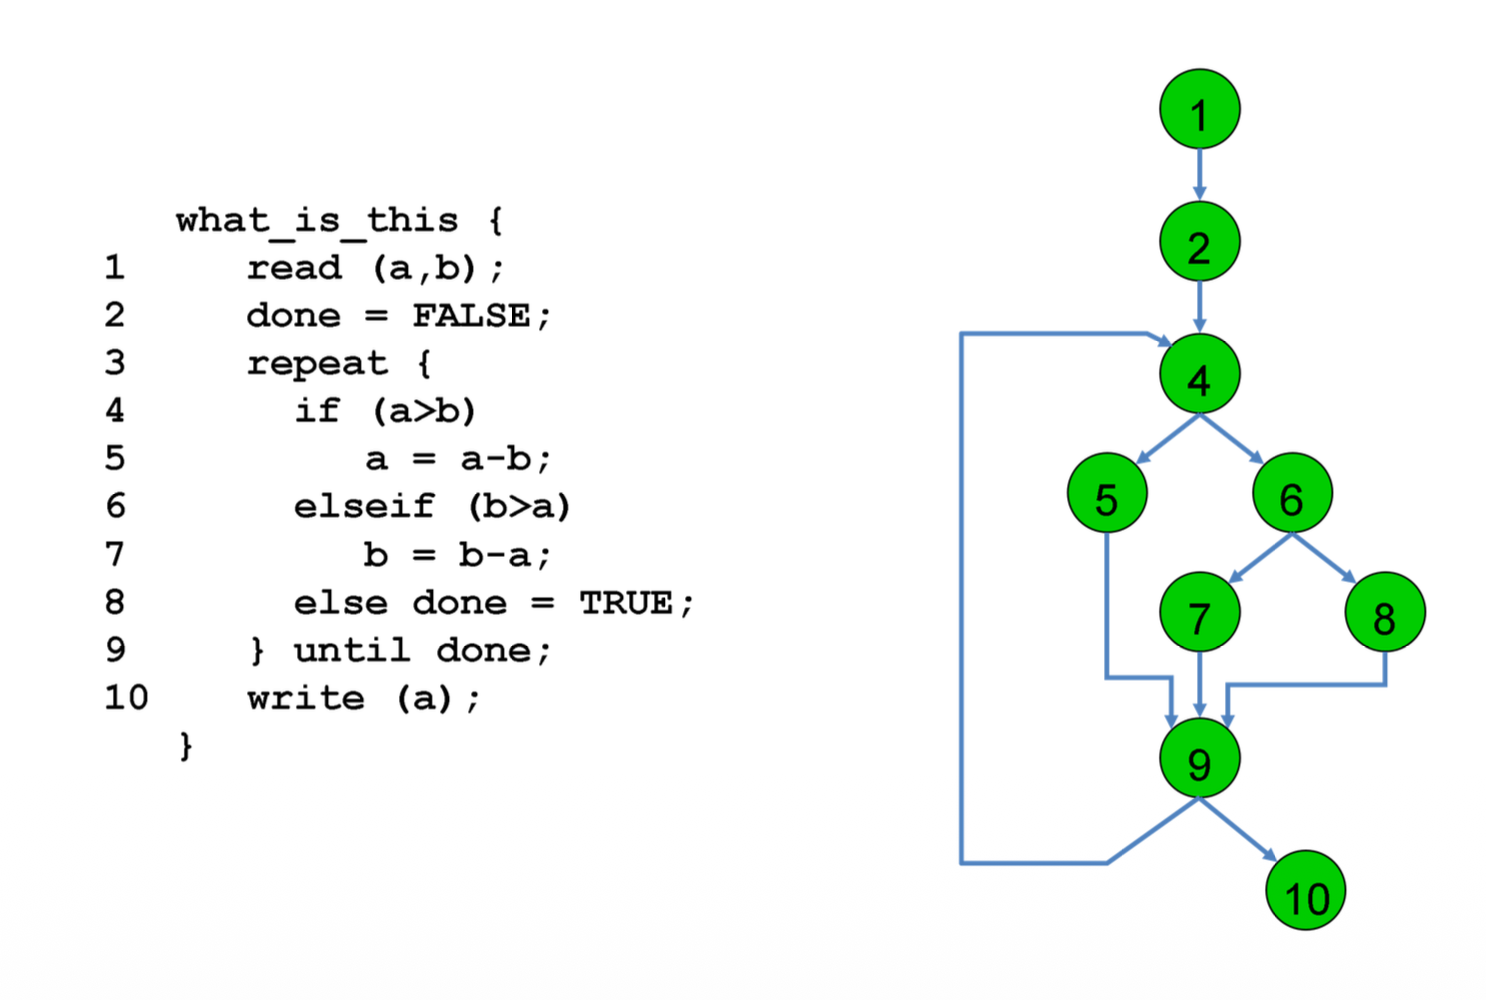
\includegraphics[width=0.5\textwidth]{images/CFG.png}
		\caption{Control Flow Graph}
		\label{fig:CFG}
	\end{center}
\end{figure}

\subsection{Sequencing Graphs}

\begin{itemize}
	\item Hierarchy of entities
\begin{itemize}
	\item entities modeling the data flow
	\item hierarchy modeling the control flow
\end{itemize}
\item Special nodes
\begin{itemize}
	\item Start/End nodes: NOP
	\item Branch nodes: BRANCH
	\item Iteration nodes: LOOP
	\item Module call nodes: CALL
\end{itemize}
\item Attributes
\begin{itemize}
	\item Nodes: computation times, costs
	\item Edges: conditions for branches, iterations
\end{itemize}

\end{itemize}

\begin{figure}[h]
	\begin{center}
	\begin{subfigure}[b]{0.40\textwidth}
		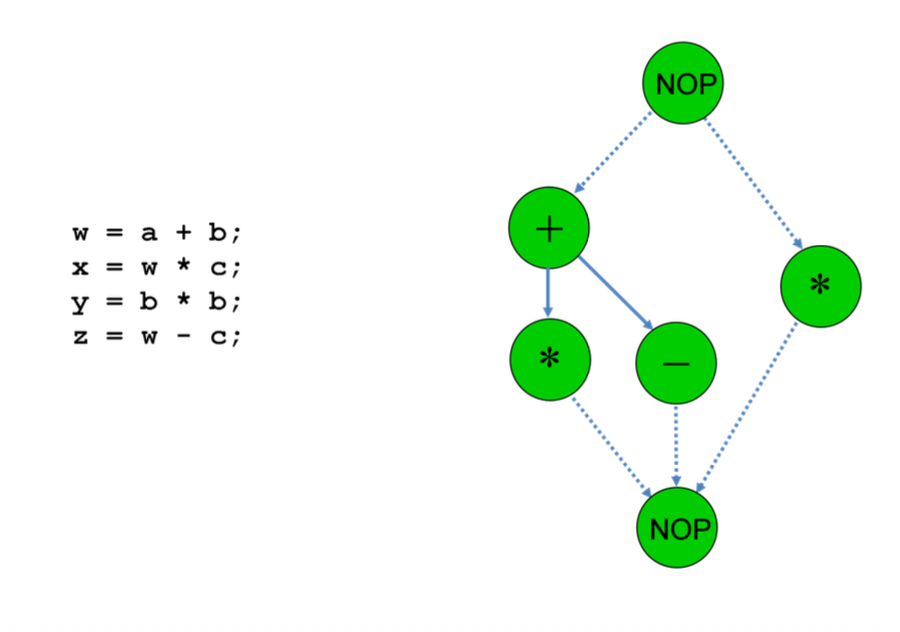
\includegraphics[width=\textwidth]{images/SG_entity.png}
		\caption{Entity}
		\label{fig:SG_entity}
	\end{subfigure}
	\hfill
	\begin{subfigure}[b]{0.50\textwidth}
		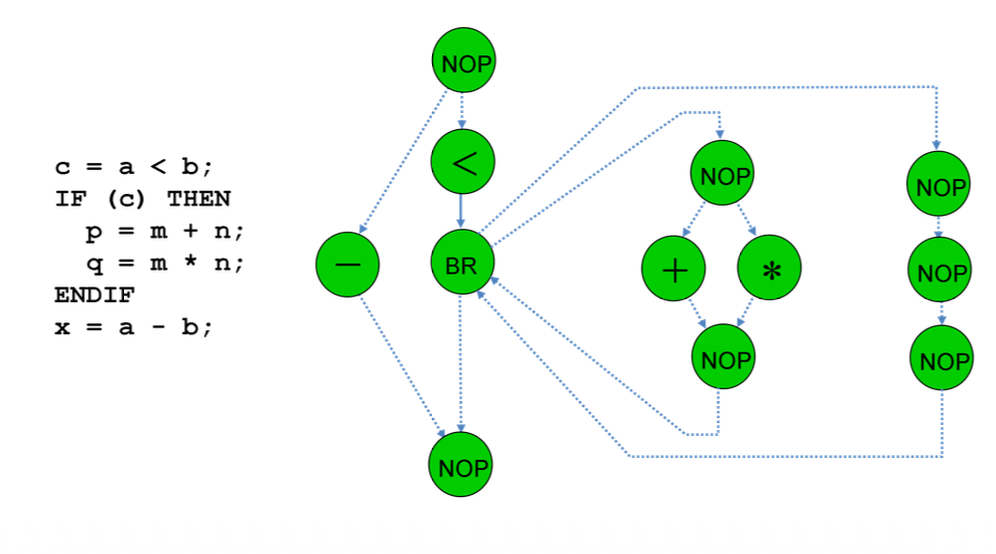
\includegraphics[width=\textwidth]{images/SG_branch.png}
		\caption{Branch}
		\label{fig:SG_branch}
	\end{subfigure}
	\begin{subfigure}[b]{0.4\textwidth}
		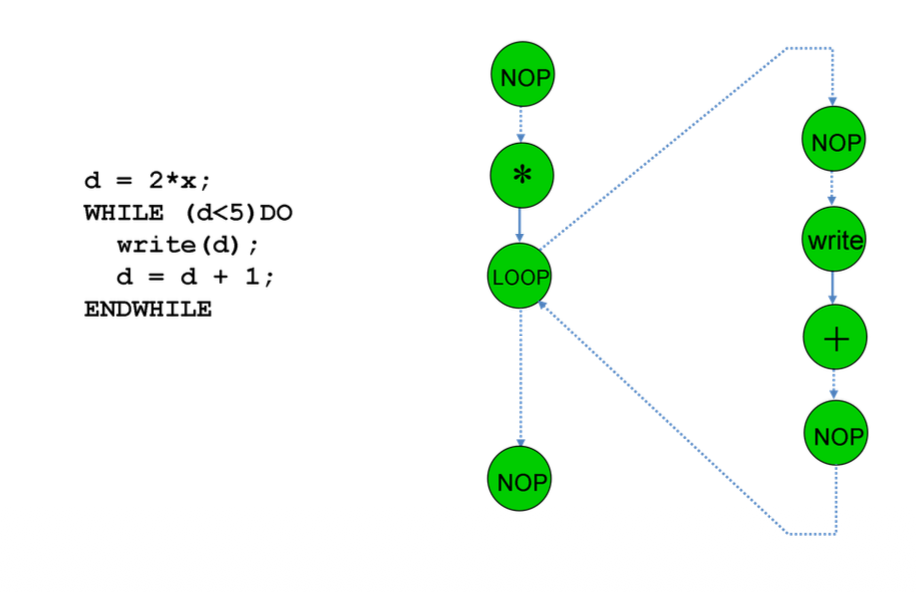
\includegraphics[width=\textwidth]{images/SG_loop.png}
		\caption{Loop}
		\label{fig:SG_loop}
	\end{subfigure}
	\hfill
	\begin{subfigure}[b]{0.5\textwidth}
		\includegraphics[width=\textwidth]{images/SG_call.png}
		\caption{Call}
		\label{fig:SG_call}
	\end{subfigure}
	\caption{Sequencing Graph}
	\end{center}
\end{figure}




